% Chapter 2

\chapter{The LHC and CMS experiment} % 
\section{The Large Hardon Collider}
\label{lhc_intro}
%LHC intro 
The LHC is a 27km circular circumference storage ring, accelerator and collider for 
both protons and Pb ions. It is situated in a stable environment in a tunnel 
100 metres underneath the Franco-Swiss boder near Geneva, Switzerland.
A double-ring synchotron, it is designed to collide proton-proton (p-p)
pairs with a centre of mass energy of up to $\sqrt(s)=14\TeV$ and a 
luminosity of up to $10^{34}cm^{-2}s^{-1}$. This makes the LHC the only collider
in operation able to directly probe $\TeV$ scale physics. 

The injected beams in the LHC are accelerated and stored for each physics run using 
a $400MHz$ superconducting cavity system. The beams of protons or pB ions 
are merged at four sections around the ring to enable collisions at interaction points.
At each of these four interaction points lies one of the four main 
experiments at the LHC; A Large Ion Collidor Experiment (ALICE) \cite{ALICE},
A Toroidal LHC Apparatus (ATLAS) \cite{ATLAS}, the Compact Muon solinoid (CMS) \cite{CMS}
and LHCb which record the collisions. Figure~\ref{LHC-diagram} shows the layout of the LHC ring including
the positions of the four main detectors. The proton beams are made up of many 'bunches' of approximately $1.1\times10^{11}$
protons localised into less than 1 ns (or 30 cm) in the direction of motion.
The beams are formed inside the Proton Synchrotron (PS) from bunches of protons 25 or 50 ns apart with an energy of 26 GeV. 
The protons are then accelerated in the Super Proton Synchrotron (SPS) to 450 GeV before being injected into the LHC at
the points shown in Figure~\ref{LHC-diagram}. Once injected into the LHC, Radio Frequency (RF) cavities 
provide around 275kW of RF power independently to each beam to accelerate the protons to allow collisions
at the operating centre of mass energy ($\sqrt(s)$). For the work contained in the thesis 
the data was taken in physics runs with $\sqrt(s) = 13\TeV$ and bunch spacings of both 25ns and 50 ns \cite{LHC}. 
The LHC operates as a storage ring for the accelerated beams using 1232 
superconducting dipole magnets in the eight arc segments. These provide magnetic fields of up to $8T$ to steer the beams. 
High precision quadropole and higher order magnets at the interacton points are used to position and focus the beams to 
maximise the occurance of high momentum collisions and therefore the luminosity. The average number of simultaneous collisions
per bunch crossing, in time pile-up (PU), for the work in this thesis was $\approx25$.
The luminosity in the LHC is not constant over a physics run, but decays due to the degradation 
of intensities and emittances of the circulating beams (mainly due to loss from collisions). Eventually,
the beam is dumped and the acceleration process is started again. An efficient turn around between
dumping the beam and the start of a new physics run of 
around 6 hours allows the luminosity collected by CMS to be maximised. 

\begin{figure}
\centering
    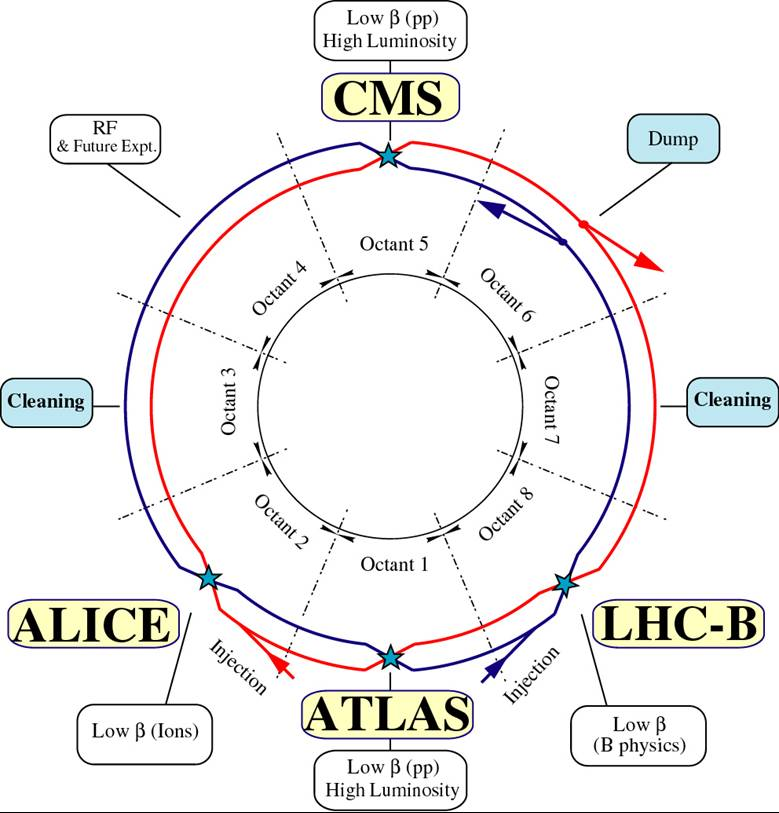
\includegraphics[width=0.8\textwidth]{./Figures/detector/lhcDiagram}
  \caption{Schematic layout of the LHC showing the position of the four main detectors as
  well as the RF systems}
  \label{fig:LHC-diagram}
\end{figure}

\subsection{LHC run condictions}

The first physics runs of the LHC from 2010-2013 (Run 1) reached energies of 3.5 and 4 TeV per beam and 
provided record-breaking integrated luminosities. The data collected allowed the 
discovery of the higgs boson \cite{higgs} as well as enabling many new regions of parameter space
to be probed. From 2013 to mid-2015 (Long Shutdown 1) the LHC was shut down for upgrade to allow design
energies to be reached. All magnet interconnectors were inspected and replaced, where necessary,
and the dipole magnets underwent a quench training programme. 

After LS1, from 2015-2016 (Run 2, which will continue up to 2018) the LHC has been running with record beam energies 
of $6.5\TeV$ per beam with bunch spacings of 25 and 50 ns. 
As shown in Figure~\ref{fig:LHC-integrated-lumi}, by the end of the 2016 run $40.7\fb$ of integrated luminosity has been 
delivered to the CMS and ATLAS detectors, with $37.5\fb$ recorded by CMS. The dataset is validated by detector
subsytem experts to ensure runs in which the data quality may be affected by any problem in one of the CMS detectors 
subsystems are excluded. The luminosity of this certified dataset is XX and it is this dataset, 
at a centre of mass energy of $\sqrt(s) = 13\TeV$, 
which is used in Chapters XX to search for Supersymmetry at the highest energy reached at a collider.

%%%FIGURE - LHC lumi plot
\begin{figure}
\centering
    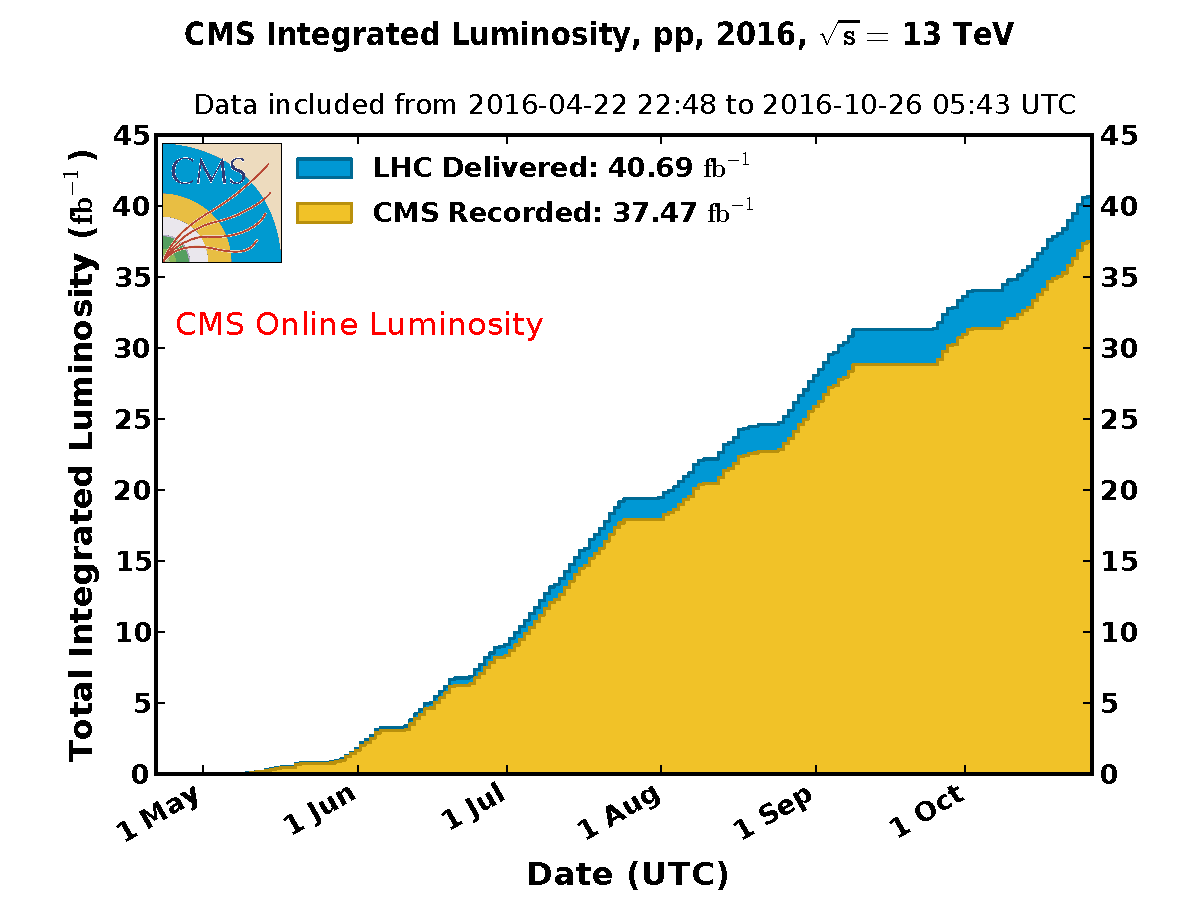
\includegraphics[width=0.9\textwidth]{./Figures/detector/int_lumi_per_day_cumulative_pp_2016OnlineLumi}
  \caption{Integrated luminosity measured online versus day delivered to (blue), 
  and recorded by CMS (orange) during stable beams and for p-p collisions at 13 TeV centre-of-mass energy in 2016.}
  \label{fig:LHC-integrated-lumi}
\end{figure}

%----------------------------------------------------------------------------------------
\section{The CMS detector}
The Compact Muon Solenoid (CMS \cite{CMS}) is one of two general purpose detectors at the LHC 
which have performed exceptionally well during the physics runs of the LHC. The main design goals
for CMS were to discover the Higgs boson as well as to search for generic models 
of new physics. To achieve this, CMS provides efficient identification and measurement
of physics objects including muons, electrons, photons, taus and hadronic showers over a
wide range of momenta and energies. Each major subsystem is made of a barrel
and two endcaps to give coverage of almost $4\pi$ in solid angle. 
This barrel design ensures global momentum imbalance can be effectively 
reconstructed, allowing the missing energy predicted in many new models of physics to be
precisely measured. A more detailed description may be found in \cite{CMS}.  

The coordinate system used by CMS takes the origin at 
the collision point. The z-axis points along the beam direction while the x-axis points radially inward
towards the centre of the LHC and the y-axis points vertically upward.
The polar angle, $\theta$, is measured from the z-axis and defines the psuedorapidity, $\eta=-ln(tan(\theta/2))$. 
This is used in preference to $\theta$ as the difference between the pseudorapidity of two 
particles is invarient under boosts along the z-axis \cite{cms_iop}. 
The eta coverage of CMS is $|\eta|<5$. The azimuthal angle, $\phi$, is defined from the x-axis in the x-y plane.
This allows the definition of $\Delta R = \sqrt{(\Delta\phi^2+\Delta\eta^2)}$, commonly used to measure the 
angular difference between objects. Transverse energies and momenta, $E_T $ and $p_T$ respectively, are defined 
as $E_T = E\sin(\theta)$ and $p_T = \sqrt{(p_{x}^2+p_{y}^2)}$. Momentum imbalances are measured as the negative 
vector sums of the momenta of the relevant objects in the x-y plane. 

\begin{figure}
\centering
    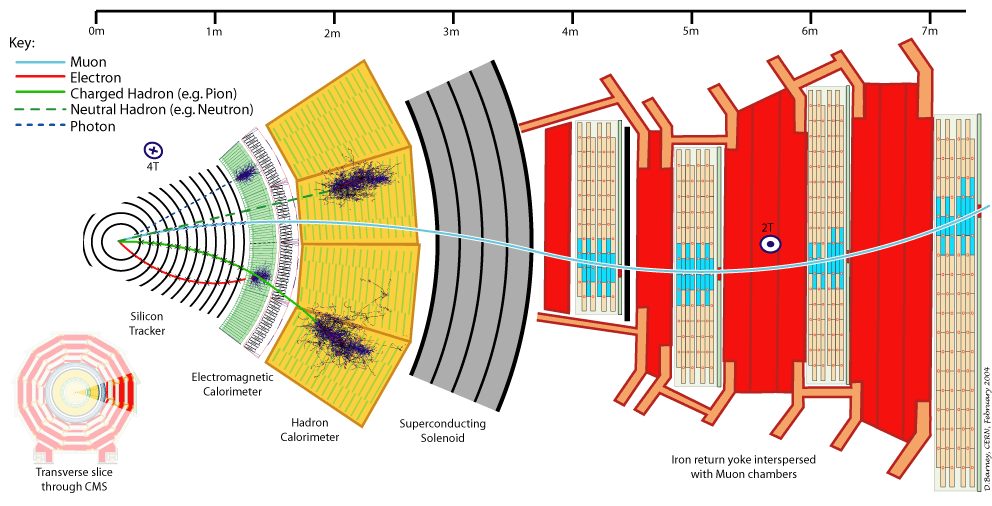
\includegraphics[width=0.9\textwidth]{./Figures/detector/CMS_Slice.jpg}
  \caption{Cross Section of CMS showing the paths of various particle types 
  through different segments of the detector \cite{cmsslice}}
  \label{CMS_SLICE}
\end{figure}

Figure \ref{CMS_SLICE} shows a cross-section of CMS in the $x-y plane$ plane as well as introducting the major detector components that will be described 
in detail in this section. The tracker lies closest to the beam and, as for the calorimetry subsystems, is situated within a magnetic field of 3.8T provided
by the superconducting solenoid. It measures the curved trajectory of charged particles through this magnetic field to determine their momenta 
as well as the location of primary and secondary vertices. The tracker is followed by the Electromagnetic Calorimeter (ECAL)
which measures energy deposited in electromagnetic showers from particles such as electrons and photons and is seperated in barrel and endcap 
components for the central and forward regions resectively. The Hadronic Calorimeter (HCAL) lies outside the 
ECAL and measures energy from nuclear interactions of hadronic particles. It is a sampling calorimeter
made up of several layers of absorber and scintillator to allow hadron showers to be measured over a maximum of around 11 radiation lengths. 
The coverage of the hadron calorimeter is extended into the forward regions with the Hadonic Forward calorimeter (HF). Enclosing the calorimetry and tracking subsystems 
is the superconducting solenoid which generates the magnetic field. Outside the solenoid, the iron return yoke lies interspersed with muon chambers, forming the outermost components of the detector. 
Muons are minimally ionising particles (MIPs), depositing little energy within the detector, and typically reach the cavern containting the detector. 
The barrel muon system is composed of drift-tubes (DT) and resitive plate chambers (RPC). In concert these provide
high resolution hit timing and positioning to determine the moun trajectory. In the forward region the DTs are replaced by cathode strip chambers 
(CSC) due to the higher radiation flux occuring along the beamline. 

\subsection{Tracker}
The CMS tracker is an all sillicon tracker with an area sensitive to charged particles of around 200$m^2$. It is designed to measure hits along the
curved trajectories of charged particles which result from the high energy p-p collisions. A cross section of the tracker in the r-z plane is shown in Fig~\ref{TRACKER_SLICE}.
The tracker has coverage for $\|\eta\| < 2.5$ and achieves an optimal efficiency in the barrel region $\|\eta\| < 0.9$ \cite{tracker_performance,tracker_tdr}. 
Close to the interaction vertex, $r < 20cm$, where the particle flux is maximal ($~10^7/s$) is the pixel detector. This system consists of an inner region of 66 million silicon 
pixels of $100\mu m \times 150\mu m$ in three overlapping layers and a forward region with two endcap discs on each side.
For $r > 20cm$ the particle flux drops to enable the use of larger silicon microstrips. These range in size from at least $10cm \times 80\mu m$ for the Inner Barrel (TIB) region 
at intermediate values of r, $20cm < r < 55cm$, to at least $25cm \times 180\mu m$ for the Outer Barrel (TOB) region ($55cm < r < 110cm$). The forward region
for r > 20cm is covered by endcap disks divided into the 9 disks of the Tracker End Cap (TEC) for the $120cm < \|z\| < 280 cm$ region and 
3 Tracker Inner Discs (TID) lying between the TIB and TEC. The TID and first 3 disks of the TEC have sensors of thickness $320\mu m$ while the remainder of the TEC disks
have sensors of thickness $500\mu m$\cite{tracker_tdr}.

\begin{figure}
\centering
    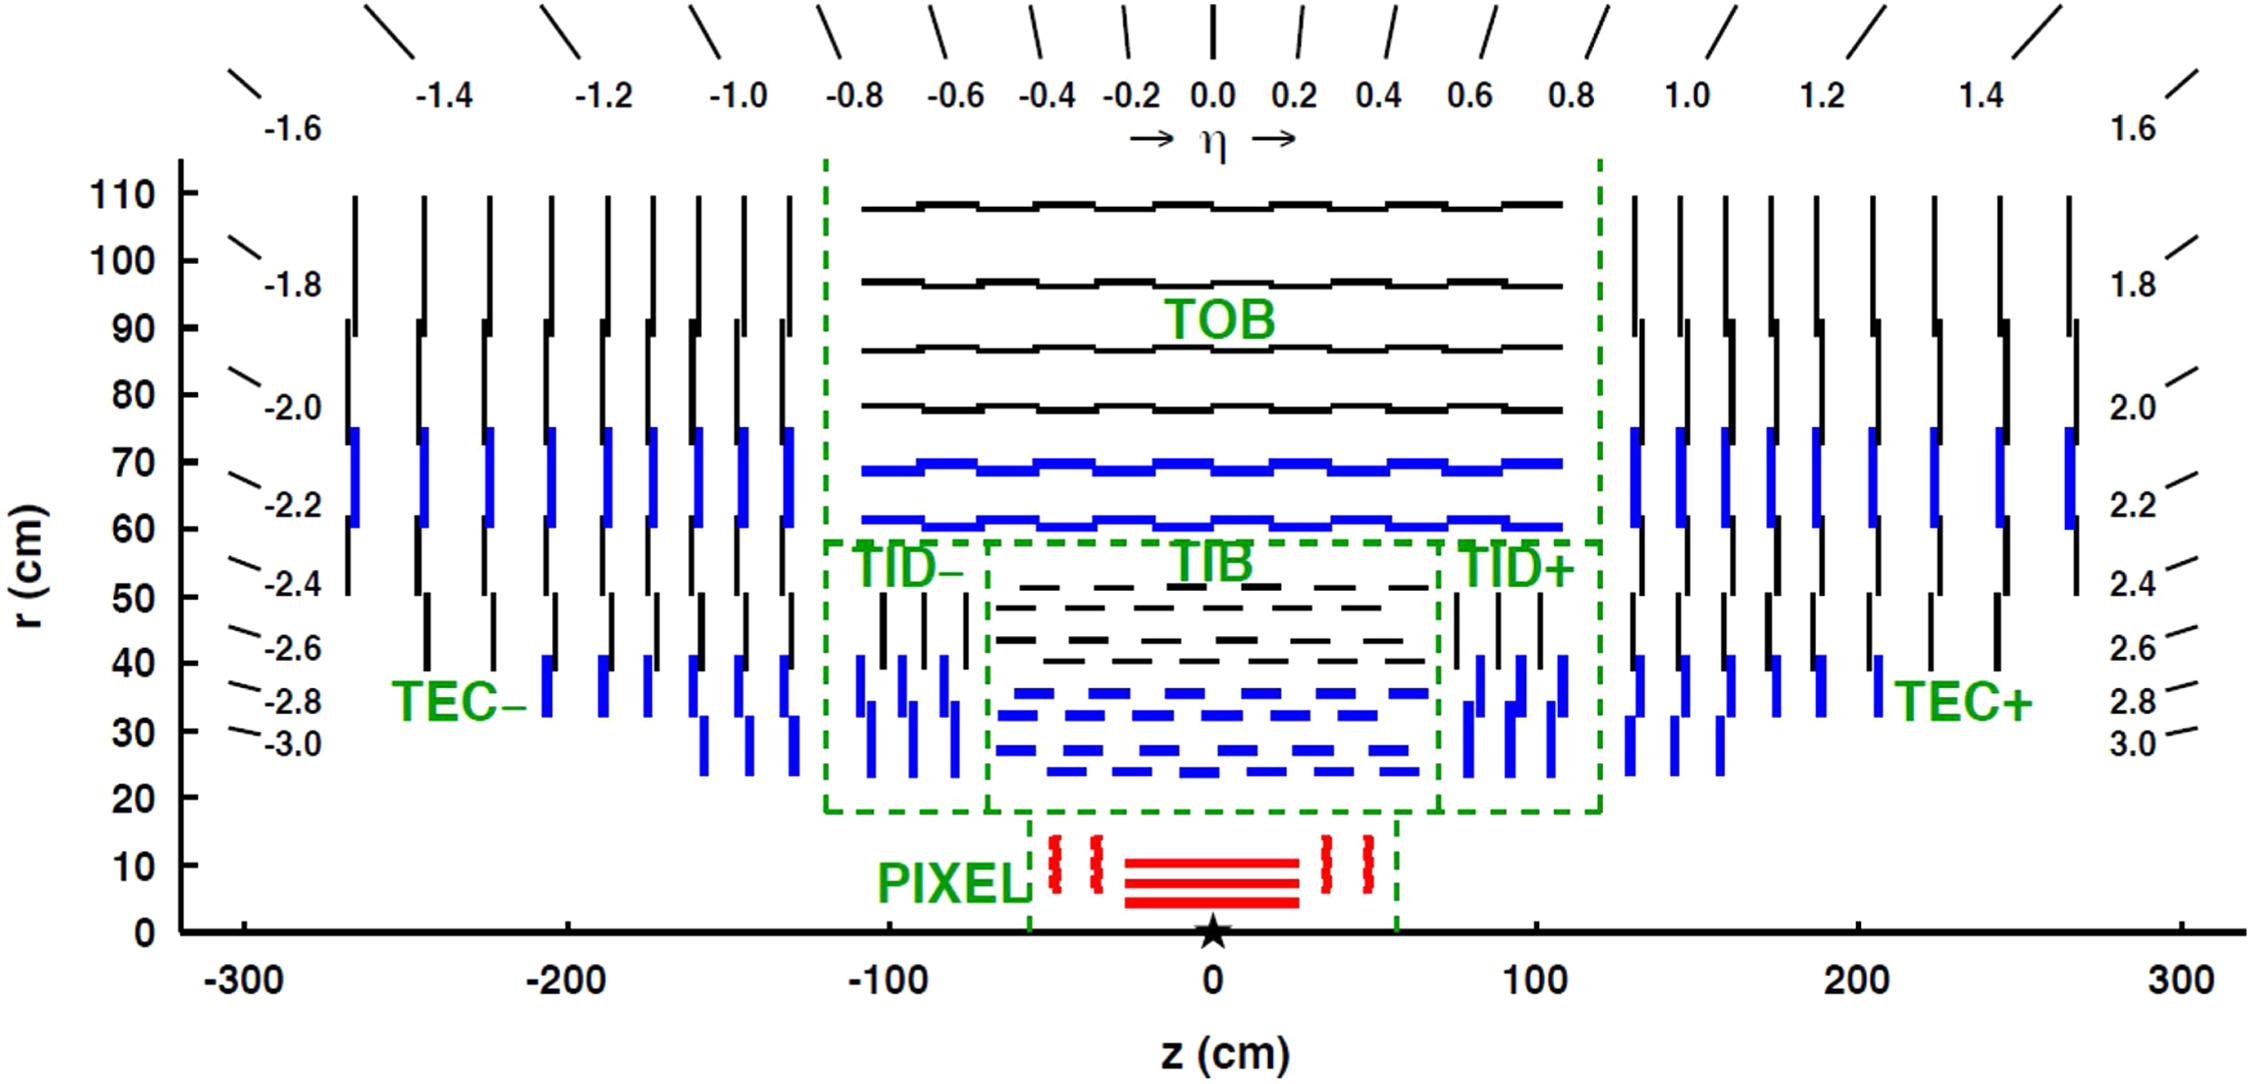
\includegraphics[width=0.9\textwidth]{./Figures/detector/CMS2Dtracker}
  \caption{A quarter cross section of the CMS tracker showing the pixel and strip components \cite{tracker_fig}}
  \label{TRACKER_SLICE}
\end{figure}

To measure the trajectories the tracker must effectively detect hits from charged particles. The efficiency for the 
hit reconstruction, defined as the fraction of particles with $p_T > 1 GeV$ passing through the fiducial regions of the sensors
in a layer for which hits are recorded, ranges from 99\% in the strip detector to 99.5\% for the pixel detector.
The position resultion for the hits also determines the track finding performance and for 
the pixel detector the resolution in the r-$\phi$ plane is $\sim10\mu m$ and $\sim20-40\mu m$ along
the z direction while the r-$\phi$ resolution for the strip detector ranges from $\sim13-47\mu m$.

\subsubsection{Tracks}

Charged particle tracks are reconstructed from the hits, considering the efficiency and resolution, 
using the iterative Combinatorial Track Finder (CTF) algorithm. The track reconstruction can be decomposed 
into four logical steps outlined below.

\begin{itemize}
\item Seeds are generated using either triplets of tracker hits or pairs of hits with an additional constraint 
from the beamspot or a pixel vertex. This gives an initial estimate of the trajectory with uncertainty \cite{tracker_early}.
\item Each seed is propagated outward through the tracker layers considering the current uncertainty in the trajectory.
In propagating, a uniform magnetic field as well as no energy loss or multiple Coulomb scattering effects are assumed.
The track parameters are then updated with the best matching hit on each layer (if any) according to the Kalman filter formalism \cite{tracker_vertex}.
The search continues until either the boundary of the tracker is reached or no more compatible hits are found. If a mimimum number
of valid hits are observed an inwards search is initiated for additional hits\cite{tracker_early}.
\item It is possible for a single charged particle track to be reconstructed more than once, starting either from different seeds or if
one seed develops into multiple track candidates. If the fraction of shared hits between two track candidates is greater
than 19\% (determined empically) the track with fewer hits is discarded. If the number of hits is equivalent the track with
 the largest $\chi^2$ is discarded\cite{tracker_vertex}.
\item After the track candidates are built and cleaned the hits in each candidate are refitted using a Kalman filter and smoother. This 
avoids possible bias from the seeding stage \cite{tracker_vertex}.
\end{itemize}

The CTF performs six iterations to determine the tracks. Between each iteration any hits that are assigned to tracks in the
previous iteration are removed from the collection. The final track collection is then filtered to remove fake tracks using 
information on the number of hits, the $\chi^2$ and the compatibilty of the track orginating from a pixel vertex. The momentum 
resolution achieved is 0.7 (5)\% at 1 (1000) \GeV in the central region\cite{tracker_early}. Using a dataset of pions and muons data from an early run 
at the LHC the tracking efficiency was measured as 98\% for tracks with $p_T > 500\MeV$ and $>99\%$ for tracks with $p_T > 2\GeV$\cite{tracker_eff}.

\subsubsection{Vertex Reconstruction}

As described in Sec.~\ref{lhc_intro}, the LHC produced an average of 25 simultaneous collisions per bunch crossing
during Run 2. It is essential to identify the Primary Vertex (PV) and the particles originating from it to allow 
particles from additional collisions to be rejected and to identify features such as displaced vertices. The tracks
are initally clustered using a deterministic annealing (DA) algorithm based on the points of closest approach of the 
tracks to the beamspot \cite{tracker_vertex}. The candidate vertices containing at least two tracks are then
fitted using an adaptive vertex fitter (AVF) to compute the best estimates of vertex parameters \cite{tracker_avf}. 
Each track in the vertex is assigned a weight between 0 and 1 corresponding to the likelihood that that track
belongs to the vertex. The tracks with weight near 1 are most consistent with the reconstructed vertex while
those that are least consistent have small weights. The number of degrees in the fit, defined as 

\begin{equation}
n_{dof} = -3 + 2 \sum_{i=1}^{\#tracks} wi,
\end{equation}

is an important parameter for distinguishing real proton-proton interactions from misclustered vertices as it is strongly corrected with
the number of tracks compatible with arising from the interaction region \cite{tracker_vertex}. The vertex
position and resolution determined using the AVF have been 
measured in early LHC data and compared with simulation as shown in Fig~\ref{fig:pvEffRes}.

\begin{figure}[hbt]
  \begin{center} 
   \subfigure[\label{fig:pvEff}]{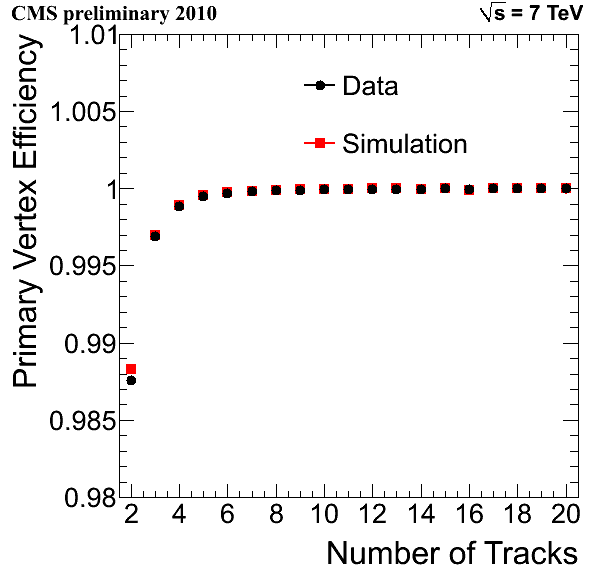
\includegraphics[width=0.5\textwidth]{Figures/detector/pvEff}}~
   \subfigure[\label{fig:pvRes}]{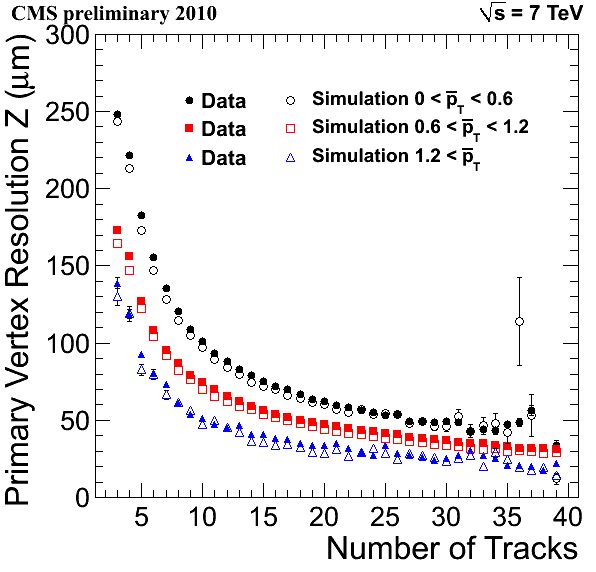
\includegraphics[width=0.5\textwidth]{Figures/detector/pvRes}}
   \caption{(a) Primary Vertex efficiency as a function of the number of associated tracks. (b) Primary Vertex 
   resolution in the z coordinate as a function of the number of associated tracks for three track $p_T$ scenarios \cite{tracker_seven}
   \label{fig:pvEffRes} }
  \end{center}
\end{figure}

The vertices are ordered according to the sum of the $p_T^2$ of the tracks associated to each vertex with the 
vertex with the highest $p_T^2$ taken as the primary vertex (PV). The position of the primary vertex can
be used for object identification and control of pile-up. Many CMS analyses, including the one in this 
thesis, make requirements that a good vertex is reconstructed from the tracks satisfying:

\begin{itemize}
\item A minimum number of degrees of freedom: $n_{dof} > 4$.
\item The collision to occur with $|z| < 24cm$ such that the primary vertex is near the interaction point in the longitudinal direction.
\item The collision to occur within a radial distance of $|d_{xy}| < 24cm$ from the beamline.
\end{itemize}

\subsection{Electromagnetic Calorimeter}

The high precision measurement of the energy and position of electrons and photons resulting from 
processes such as Higgs decay is an important design goal of the CMS experiement. Additionally,
a substantial energy fraction of jets, which are central to the analysis outlined in this
thesis, is formed of photons whose properties cannot be measured in any other subsystem.

The CMS ECAL is formed of high density lead tungstate ($PbWO_4$) crystals encorporating a barrel section (EB) 
and two endcaps (EE) outside the tracker \cite{ecal_tdr}. The high density (8.28 $g/cm^3$), short radiation length (0.89cm) 
and small Moliere radius (2.2cm) of the crystal are optimal for a compact calorimeter with high granularity. In addition the 
crystals are radiation hard (up to 10 Mrad) and have a fast scintillation decay time (80\% of the light is emmited within 25ns)
comparable to the smallest bunch spacing provided by the LHC. 

The EB has an inner radius of 129 cm and covers the range $|\eta| < 1.479$. The crystals are arranged into 36 
identical 'supermodules' which surround the beam line in a quasi-projective geometry (the gaps between
crystal modules are offset by $3^\circ$ with respect to the line from the nominal vertex position)
and cover $0.0174$ in $\Delta\phi$ and $\Delta\eta$ \cite{CMS}. The crystals have a front face cross-section 
of $\sim 22\times22mm^2$ and a length of $230\mm$. This allows electrons and photons to deposit most of their  
energy within a single crystal as the crystals have a depth equivalent to 25.8 radiation lengths and 
a breadth comparable to the Moliere radius. 

The endcaps lie at a distance of 314 cm from the vertex and cover the range $1.479 < |\eta| < 3.$. The crystals
are structured into 2 'Dees' which consist of semi-circular aluminium plates upon which structural units of 
$5\times5$ 'superclusters' of crystals are cantilevered. Similarly to the EB, these are arranged off-axis from
the nominal vertex position. The identical crystals have a front face cross section of 
$\sim 28.6\times28.6 mm^2$ and a length of $220\mm$ (24.7 radiation lengths) \cite{CMS}.

The energy of the incoming electromagnetic particles is measured through the scintillation light produced
in the crystals. The light yield of the crystals is reasonably low ($30\gamma/\MeV$)
and so photodiodes with intrinsic gain that can operate within a magnetic field must be used to collect 
the scintillation light and amplify the signal \cite{ecal_tdr}. Silicon avalanche photodiodes (APDs) are used as photodetectors
in the barrel region while vacuum photo-triodes (VPTs) are used in the endcaps due to their lesser sensitivity
to the high radiation conditions in the forward regions. The temperature sensitivity of both the crystals 
and phododiodes requires a stable temperature of $\sim291K$ with a target stability of $0.1K$. 

The final component of the ECAL is the preshower which covers much of the endcaps ($1.653 < |\eta| < 2.6$). In addition
to its principle aim of identifying neutral pions it assists in the identification of electrons against MIPs and with
the position determination of electrons and photons. The preshower is a sampling calorimeter with two layers with each layer
consisting of a lead radiator which initiate electromagnetic showers (of thicknesses equal to 2 and 1 radation lengths for the 
first and second layer respectively) in front of silicon strip detectors which 
measure the energy deposited and transverse shower profile \cite{ecal_tdr}.  

The energy resolution of the ECAL can be parameterised as the summation of three independent sources as shown 
in Equation~\ref{equ:energy-resolution} \cite{ecal_performance2},

\begin{equation}
\frac{\sigma_E}{E} = \frac{a}{\sqrt{E(\GeV)}} \oplus \frac{b}{E(GeV)} \oplus c^2,
\label{equ:energy-resolution}
\end{equation}

where the parameters $a$, $b$, $c$ are the stochastic, noise and constant contributions respectively. These have been
derived from an electron beam test as $a=2.8\%$, $b=12\%$ and $c=0.3\%$. The stochastic
term is very low as the shower is mainly contained within each crystal. The noise term is determined mainly by 
the preamplifier and pileup effects while the constant term originates mainly from intercalibration errors and crystal non-uniformity \cite{ecal_tdr}. 
In physics runs additional effects due to radiation damage or material upstream of the beam must be controlled to a 
fraction of a percent \cite{ecal_performance}. The high resolution achieved by the CMS ECAL allows effective identification and energy measurement of electrons and photons, crucial to
controlling electroweak backgrounds in the analysis described in this thesis.

\subsection{Hadron Calorimcter}

The HCAL is a sampling calorimeter which is designed to measure the hadronic properties of jets as well as provide good 
containment and hermicity for ensuring momentum imbalance from neutrinos or new physics particles can effectively measured \cite{hcal_tdr}.
These quantities are critical for the analysis described in this thesis.
The design of the HCAL is largely determined by the space limitations due to the ECAL at $r = 1.77 m$ and the solenoid at $r = 2.95 m$.
Having the main body of the HCAL within the magnet allows the particle flow (PF) jet algorithm, described in Section ??, to have maximum 
efficacy. 

The central region of the HCAL is formed by the HCAL Barrel (HB) covering the region $|\eta| < 1.3$ which sits between
the ECAL and magnet. Brass is used as the absorbed material due to its relatively short interaction length (16.42cm), ease of machining 
and because it is non-magnetic. The space taken by the active material is minimised through the use of plastic scintillator tiles
read-out with embedded wavelength-shifting (WLS) fibres \cite{CMS}. The detector is made up from 36 identical azimuthal wedges split into two barrels.
The active scintillator tiles are divided into 2304 segments (towers) each covering $\Delta\phi \times \Delta\eta = 0.087 × 0.087$, corresponding to the 
same area taken by the $5\times5$ ECAL superclusters. The HB is extended to $ 1.3 < |\eta| < 3.$ by the HCAL Endcap (HE). This is formed of 14 layers 
with the first 6, covering  $|\eta| < 1.74$, made from towers of $\Delta\phi \times \Delta\eta = 0.087 × 0.087$. For $|\eta| > 1.74$ the $\Delta\phi$
size is $0.174$ while the $\Delta\eta$ increases from 0.9 to 0.178.

The Hadronic Outer (HO) sits outside the magnet in the region $|\eta| < 1.26$ and is designed as a 'tail-catcher'.
It increases the effective thickness of the HCAL to over 10 interaction lengths, reducing the tails in the energy resolution
as well as improving the \met resolution. It is composed of iron absorbers and scintillator layers (with the same tile geometry as in the HB), divided into 
12 $30^\circ$ sections \cite{hcal_tdr}. 

Finally, coverage for $3. < |\eta| < 5.$ is provided by the Hadronic Forward (HF) installed $11.2 m$ from the interaction point. This provides
excellent measurement of forward hadronic activity as well as hermitacy for \met measurements \cite{hcal_tdr}. The HF is composed of a 1.65m thick steel absorber 
embedded with a grid of $0.6 mm$ quartz fibres, each separated by $5mm$, running parallel to the beam. The energy is measured using the Cherenkov
light produced by particles, formed in the hadronic shower, travelling within the fibres. The HF is segmented into 13 towers in $\eta$ with a
size of $\Delta\eta \approx 0.175$, except for the lowest $\eta$ tower with $\Delta\eta \approx 0.1$. The azimuthal segmentation of all towers is 
$\Delta\phi = 0.175$, except for the highest $\eta$ tower with $\Delta\phi = 0.349$.

Similarly to the ECAL, the HCAL resolution was measured using a test beam of single charged pions to be given by the expression shown in Equation~\ref{equ:energy-resolution-hcal} 
\cite{hcal_performance},

\begin{equation}
\frac{\sigma_H}{E} = \frac{94.3\%}{\sqrt{(E)}} \oplus 8.4\%.
\label{equ:energy-resolution-hcal}
\end{equation}

\subsection{Solenoid Magnet}

The design specifications of the solenoid magnet are driven by the desire to unambiguously determine
the sign of muons with momentum $\sim 1\TeV$. This requires a resolution of $~10\%$ at $p=1\TeV$.
To achieve this, the CMS experiment uses a Niobium-Titanium superconducting magnet with length 
12.5m and a diameter of 6m which can operate up to fields of 4T. A field of 3.8T provides
sufficient bending power achieve the design goal and so, to maximise its lifetime, the magnet is
typically run at this field strength \cite{CMS}.

\subsection{Muon System}

Effective identification and measurement of muons is critical to the design goals of the LHC and
for the analysis described in this thesis. Centrally produced muons are measured three times:
in the inner tracker, after the coil and in the return flux. Three types of detectors which rely of gas ionisation are 
used to identify and measure muons -- drift tubes (DTs), Cathode Strip Chambers (CSCs) and Resistive
Plate Chambers (RPCs) \cite{CMS}. DTs are used in the central barrel region of $|\eta| < 1.2$ where 
the neutron induced background is small, the muon rate is relatively low, 
and the magnetic field is low (~0.4T) and uniform. In the endcap region of $ 1.2 < |\eta| < 2.4$ these conditions are 
reversed and CSCs are used. RPCs are used in both the barrel and endcap region (covering the range $|\eta| < 1.6$) as they provide a fast response with a good time 
resolution, allowing the bunch crossing to be unambiguously resolved, but much coarser position resolution than the DTs or CSCs \cite{muon_tdr}. 
The configuration of the muon systems is shown in Fig~\ref{MUON_SLICE}.

\begin{figure}
\centering
    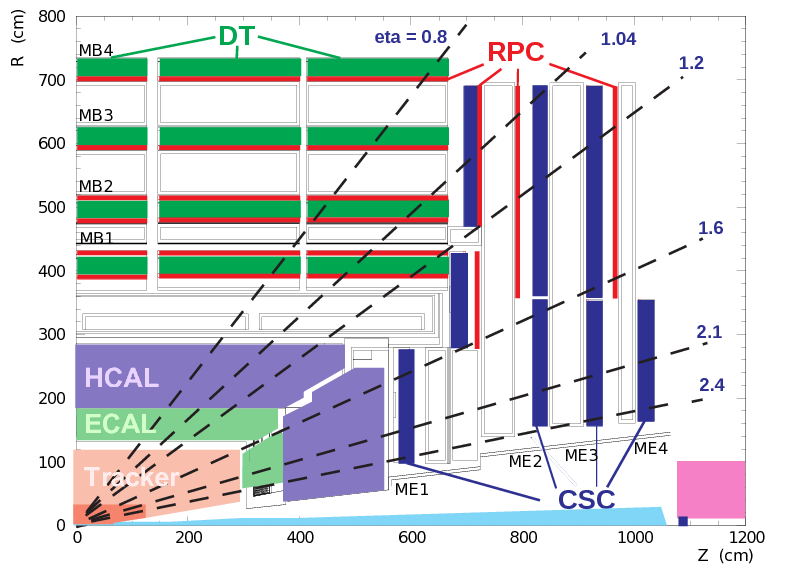
\includegraphics[width=0.9\textwidth]{./Figures/detector/muon_sys}
  \caption{A quarter cross section of the CMS muon system showing the DTs in the barrel region ($|\eta| < 1.2$) and the CSCs in the endcap
  region $ 1.2 < |\eta| < 2.4$. RPCs are layered with the DTs and CSCs in the range $|\eta| < 1.6$ to provide an independent but complementary measurement \cite{CMS}.}
  \label{MUON_SLICE}
\end{figure}

The performance of the muon system has been measured using early 7 \TeV beam and cosmic muon data \cite{muon_performance}. 
The efficiency of muon reconstruction is typically 96-99\%. The muon system relies on the effective
absorption of charged particles other than muons in the layers of the detectors.
`Punch through' of such particles is reduced to $\sim 5\%$ for the first muon station and to
$\sim 0.2\%$ for further stations. The resolution for muon momentum measurement
was measured as $\sim 1.8\%$ ($10\%$) for muons of $\pt=20\GeV$ ($\pt=1000\GeV$) using 7 \TeV~beam and cosmic muon data. 



% \begin{description}
% \item[Silicon Tracker]The job of the tracker is to measure the momentum of charged particles from their path through a magnetic field \cite{siliconTDR}. The CMS tracker achieves $10\mu m$ accuracy with coverage for $|\eta|<2.5$ and has a resolution of 1\%.
% \item[Electromagnetic Calorimeter (ECAL)] The ECAL measures the energy of incident photons and electrons. The ECAL barrel is made of 61,200 $PbWO_4$ crystals and provides coverage for $|\eta|<1.48$ \cite{ecal}. This is extended to $|\eta|<3$ by the endcap which adds another $10764$ crystals. The endcap has a pre-shower to distinguish between $\gamma$ and $\pi^0$. The ECAL has a resolution of 0.5\%.
%  \item[Hadronic Calorimeter (HCAL)] The HCAL is made from alternating brass and scintilator layers with a coverage of $|\eta|<3.0$ \cite{hcal}. The coverage is extended to  $|\eta|<5.0$ by an iron/quartz forward calorimeter \cite{hfhcal}. The average resolution is 11\%. 
%  \item[Muon Chambers]The muons are not stopped by any of the calorimeters and therefore require a separate detector with coverage $|\eta| < 2.4$. The muon chambers are interspersed with the magnet return yoke. The high magnetic field allows for accurate momentum measurement \cite{muons}. The resolution is 1\%.
% \end{description}
% As the data rate ($40Mhz$) is far too high for every event to be stored and as new physics will only 
% be seen in a minority of events a trigger system for interesting events is necessary. 
% This happens in two stages: the L1 Calorimetric and Muon Trigger (Hardware) and the High Level Trigger (Software) \cite{HLT}. 
% The L1 trigger must operate within $\mathcal{O}10ns$ and so  the calorimetric trigger only takes input
% from the ECAL and HCAL. This is described in more detail in chapter \ref{Chapter3}. The input from the
% L1 triggers is then combined in the Global Trigger (GT) which decides whether to keep the event. 
% The $\mathcal{O}100kHz$ events which pass L1 selection are processed in the HLT which utilises the 
% calorimeter information along with tracking and the muon system to further reduce the rate to $\mathcal{O}1kHz$.
